
\setchapterimage[6cm]{cabecera}
\setchapterpreamble[u]{\margintoc}

\chapter{Procesos e Hilos}  
\label{ch:Pro-Hil}
\index{procesos e hilos}
Las computadoras son sistemas o dispositivos capaces de ejecutar procesos.  
 Los \gls{procesos} son programas ejecutándose dentro de su propio espacio de direcciones. Se puede decir que un proceso es un supervisor de \gls{hilos} de ejecución. Un hilo es una secuencia de código en ejecución dentro del contexto de un proceso. \cite{Steen2017}

Un proceso consta de un \gls{entorno de ejecucion} junto con uno o más subprocesos o  hilos. Un hilo es la abstracción del sistema operativo de una actividad. Un entorno de ejecución
consiste principalmente en \cite{Coulouris2011}:
\begin{itemize}
	\item  un espacio de direcciones;
	\item sincronización de subprocesos y recursos de comunicación como semáforos e interfaces de comunicación (por ejemplo, sockets);
	\item recursos de nivel superior como archivos abiertos y ventanas. Los entornos de ejecución normalmente son costosos de crear y administrar, pero varios hilos pueden compartirlos, es decir, pueden compartir todos los recursos accesibles dentro de ellos.
\end{itemize}
 
%%%%%
 
Entre las ventajas que tiene el uso de hilos en procesos centralizados podemos indicar las siguientes. Los hilos comparten el mismo espacio de direcciones. El cambio de \gls{contexto de hilos} puede ser hecho independiente del sistema operativo. Por su parte, el cambio de proceso es más costoso ya que implica poner el sistema operativo en el bucle, es decir, bloquear el kernel. El uso de hilos permite evitar el cambio de procesos, se  estructura las  aplicaciones, no como una colección de procesos sino a través de múltiples hilos.

Otra ventaja es que ayuda en la exploración del paralelismo, en  un proceso de hilos múltiples, los hilos pueden ser programado para ejecutarse en paralelo en un procesador multiprocesos o multinúcleo. 
				

%-------------------------------------------------
%\section{Hilos en Sistemas Distribuidos } 
\section{Clientes Multihilos}  \index{multihilo}

En el contexto de arquitecturas cliente-servidor, la implementación de hilos en el lado del cliente  proporciona los siguientes beneficios: 
 
		\begin{itemize}		
 
			\item   Ocultar latencias de red: El navegador web escanea una página HTML entrante y encuentra que hay más archivos que necesita, entonces  continúa con el proceso de recuperación de los mismos. Los archivos recuperados se despliegan conforme van llegando. De esta manera, el usuario no necesita esperar hasta que todos los componentes de la página sean recuperados por completo.
			
			\item Cada archivo es recuperado por un hilo: La programación de la configuración de una conexión y la lectura desde el servidor pueden llevarse a cabo mediante una  solicitud de tipo HTTP(bloqueo). Las llamadas de este tipo no suspende el proceso por completo.
			
			\item   Conexiones simultáneas:
			 	Cuando se utiliza cliente multihilos, las conexiones pueden configurarse como réplicas diferentes lo cual permite que los datos sean transferidos en paralelo asegurando efectivamente que se despliega 	la página web completa en un tiempo más corto que con un servidor no replicado.
		\end{itemize}        
 

\marginnote[-5cm]{
	\begin{kaobox}[frametitle={Ejemplo: Múltiples llamadas a RPC}  ]
	 Un cliente realiza varias llamadas al mismo tiempo a procesos remotos, cada una por una diferente hilo. 
	 Luego, espera hasta que se hayan devuelto todos los resultados. Si  las llamadas son a diferentes servidores, podemos tener una rapidez lineal en la respuesta a la solicitud.
	\end{kaobox}
}
	 
 

	
	\paragraph{Interfases de Usuario en la Red} 
	\index{interfases de usuarios}

     Las interfases de usuario en la red pueden implementarse a nivel de aplicación y a nivel de middleware.
	
	 \begin{figure} %
		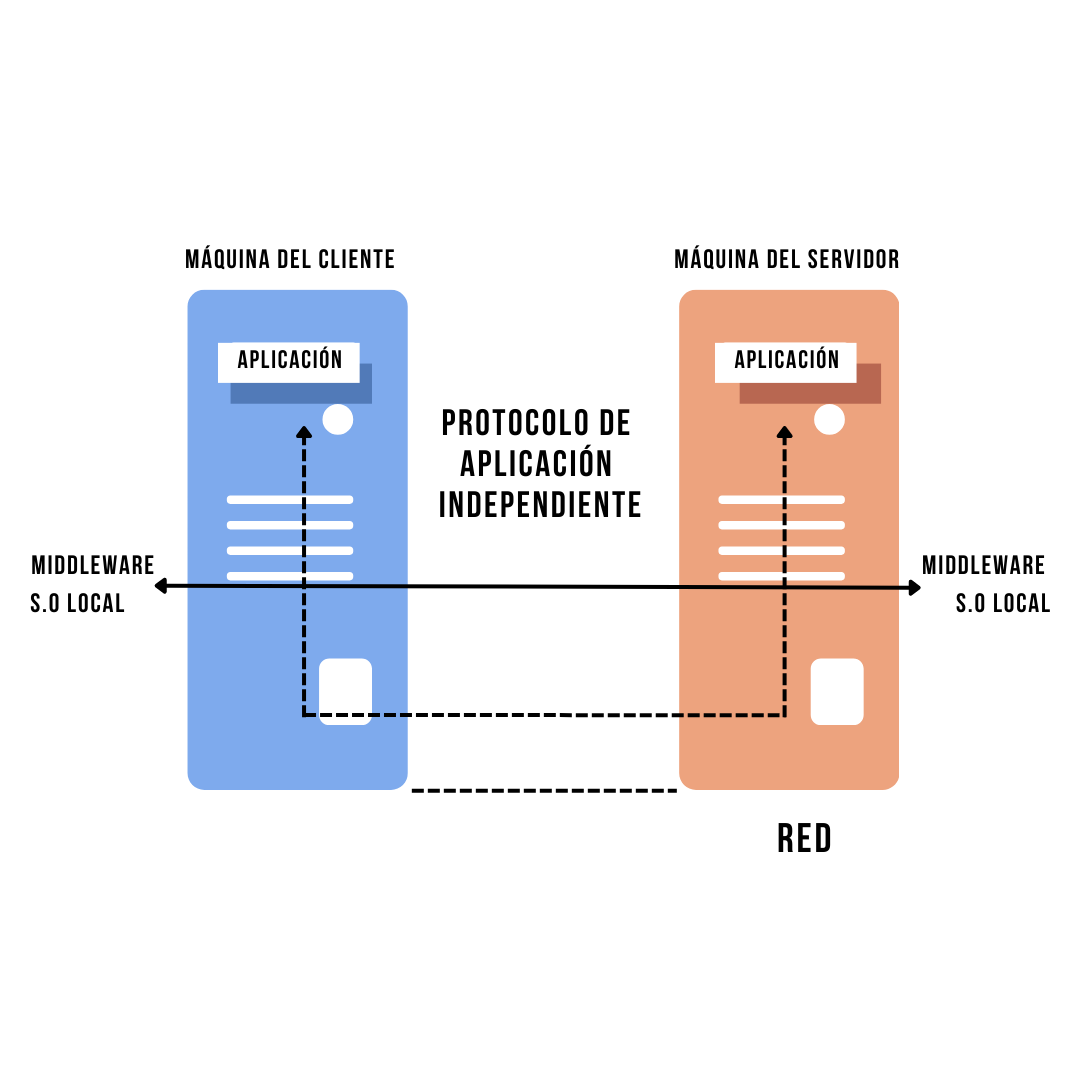
\includegraphics[width=0.4\linewidth]{3/11}
		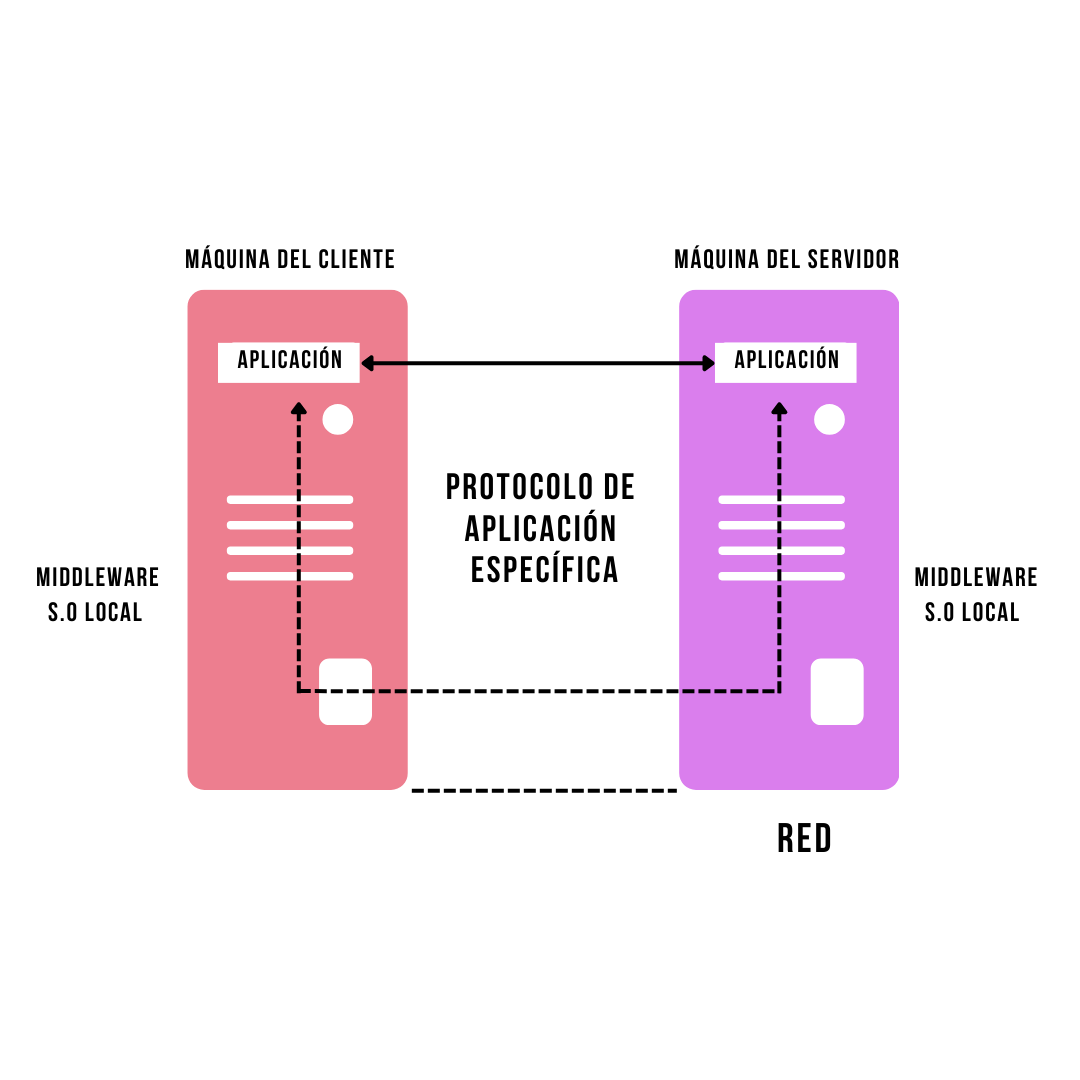
\includegraphics[width=0.4\linewidth]{3/12}
		\caption{(a) Aplicación en red con su protocolo. (b) Aplicación con acceso a  aplicaciones remotas. Adaptado de \ST}
		\label{fig:Clientes-Hilos}
	\end{figure}
	 
	
	Este ejemplo,  tomado de \sidecite{Steen2017}, ilustra la diferencia de la implementación de interfases a nivel del cliente o en el middleware. Aqui se ilustra el comportamiento de una agenda que se ejecuta en una PDA de un usuario  y que requiere sincronizarse con una agenda compartida remota. En este caso, un protocolo a nivel de aplicación manipulará esta sincronización, como podemos ver en la figura \ref{fig:Clientes-Hilos} parte (a). En la parte (b) de la mencionada figura se muestra una  solución donde se proporciona acceso directo a servicios remotos solamente por medio de la oferta en la interfaz de usuario. Esto significa que la máquina cliente sólo se utiliza como terminal sin necesidad de almacenamiento local. En este caso de interfaces de usuario en red, todo es procesado y almacenado en el servidor. Este método de \gls{cliente ligero} llamado también clientes delgados, recibe mayor atención al incrementarse la conectividad a internet, y a medida que los  dispositivos portátiles (\textit{hand-held}) se han vuelto más sofisticados. 
	
	
	%------------------------------------------------
	\paragraph{Software del lado del Cliente para transparencia en la distribución}   
	%-----------------------------------------------
	  Un cliente no solo consta de una  interfaz de usuario y de la aplicación, el software   del cliente tiene los componentes necesarios para lograr la transparencia  en el acceso, migración, distribución y fallas. A continuación se menciona cada una de este tipo de transparencia \sidecite{Steen2017}:
	 
	\begin{itemize} 
		
		\item Transparencia de acceso: Implementando \textit{stubs} (apéndices o conectores) del lado del cliente para las llamadas a procedimientos remotos (RPC). La transparencia en el  acceso es gestionada  a partir de una definición de interfaz donde se muestra lo que el cliente tiene que ofrecer. 		
				
		\item Transparencia de ubicación/migración: deje que el software del lado del cliente realice un seguimiento de ubicación actual. Para ello es importante el uso de un adecuado sistema de nombres, ver la sección referida al DNS en \ref{ch:arq-SD}. 
		
		\item Transparencia de replicación: múltiples invocaciones manejadas por el código auxiliar del cliente.  El software del lado del cliente puede recopilar de manera 	transparente todas las respuestas y pasar solamente una respuesta a la aplicación del cliente. Esquema  de este comportamiento se muestra en la  figura \ref{fig:Clientes-transp}.
		
		 \begin{figure} %
			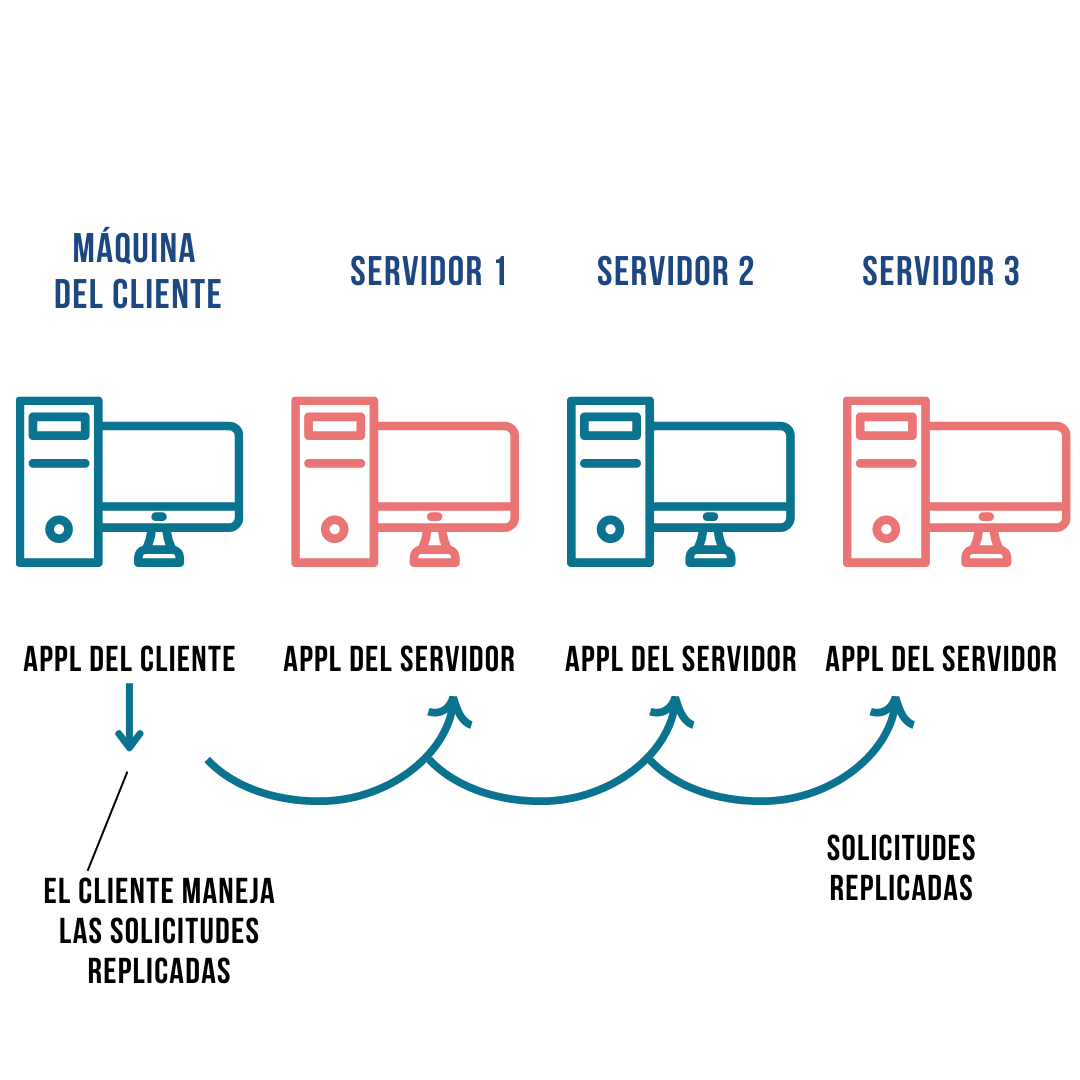
\includegraphics[width=0.8\linewidth]{3/13.png}
 			\caption{Transparencia de replicación de un servidor mediante una solución
 				del lado del cliente. Adaptado de \ST}
			\label{fig:Clientes-transp}
		\end{figure}
		 
		\item Transparencia de falla:  El enmascaramiento de las fallas de la comunicación con un servidor se hace a través del middleware del cliente:  ejemplo,   la 	configuración del \textit{middleware} del cliente para intentar repetidamente la conexión a un servidor, o  tratar con otro servidor después de varios intentos fallidos; también cuando middleware del cliente devuelve datos que tenía en caché durante una sesión previa. 
	\end{itemize}
	
	
%-------------------------------------------------	
%------------------------------------------------- 
%-------------------------------------------------

\section{Servidor Multihilos}
\index{servidor multihilos}

%-------------------------------------------------
 El uso de clientes multihilos presenta  importantes beneficios para los sistemas distribuidos, pero el uso  principal  de la tecnología multihilos está del lado del servidor.
 Veamos sus caracter\'isticas.
 
	\paragraph{Ventajas y desventajas}
	El uso de hilos en el lado del servidor proporciona las siguientes ventajas que redundan en la mejora del rendimiento  para las aplicaciones distribuidas:

		\begin{itemize}	 	
		     	
			\item Iniciar un hilo es más barato que comenzar un nuevo proceso. 			
			\item Tener un servidor multihilos evita la ampliación a un sistema con  multiprocesadores.
		    \item Un hilo no afecta a otros hilos. En un servidor multihilos, si se produce algún error en cualquiera de los hilos, ningún otro hilo se verá afectado, todos los demás hilos seguirán ejecutándose con normalidad. En un servidor de hilo único, todos los demás clientes tenían que esperar si ocurría algún problema en el hilo.	
			\item  Al igual que con los clientes: oculta la latencia de la red reaccionando a la siguiente solicitud mientras la anterior está siendo respondida.     
		    \item 	Rápido y eficiente: el servidor multihilo podría responder de manera eficiente y rápida a las crecientes consultas de los clientes rápidamente.
		    \item 	El tiempo de espera para los usuarios disminuye: en un servidor hilo único, otros usuarios tenían que esperar hasta que se completara el proceso en ejecución, pero en servidores multihilos, todos los usuarios pueden obtener una respuesta a la vez, por lo que ningún usuario tiene que esperar a que finalicen otros procesos.	 
		\end{itemize}        
 
 
     Pero las ventajas relevantes descansan en que proporciona aplicaciones mejor estructuradas ya que simplifica el flujo de la información:

		\begin{itemize} 
			\item  La mayoría de los servidores tienen altas demandas de solicitudes  E/S. Con las  llamadas con bloqueos, se simplifica la estructura general de la aplicación. 
			
			\item  Los programas multihilos tienden a ser más pequeños y fáciles de entender debido a que se simplifica el flujo de la informaci\'on.
		\end{itemize}
		

	
		
	Las desventajas de esta arquitectura:
	\begin{itemize}
		\item Código complicado: puede resultar difícil escribir el código del servidor multihilo. Estos programas no se  crean fácilmente.
		\item La depuración es difícil: analizar la razón principal
			 y el origen del error no es fácil de seguir.
	\end{itemize}
 
 
%-------------------------------------------------
 
	\paragraph{Organización del servidor multihilo }
	
 
En la figura \ref{fig:serv-multi} se ilustra la  organización de un servidor multihilos. El servidor  espera una petición de entrada para una operación de  archivo, posteriormente ejecuta la petición, y luego envía la respuesta de regreso. En la figura \ref{fig:serv-multi}, un hilo servidor, lee las peticiones  de entrada para una operación con archivos. Las peticiones son enviadas por clientes hacia  un puerto   conocido por este servidor. Después de examinar la petición, el hilo en el servidor elije  un hilo trabajador sin utilizar (desbloqueado) y le asigna la petición.
 
 El hilo trabajador procede a realizar una lectura con acción de bloqueo en el sistema de archivos local, ello puede  provocar que el hilo se suspenda hasta que los datos sean recuperados desde el disco local. Si el hilo  se suspende, se puede selecciona otros hilo para su ejecución. Por ejemplo, el hilo servidor puede seleccionar la adquisición de más hilos trabajadores. 
 
 
	
	 \begin{figure} %
		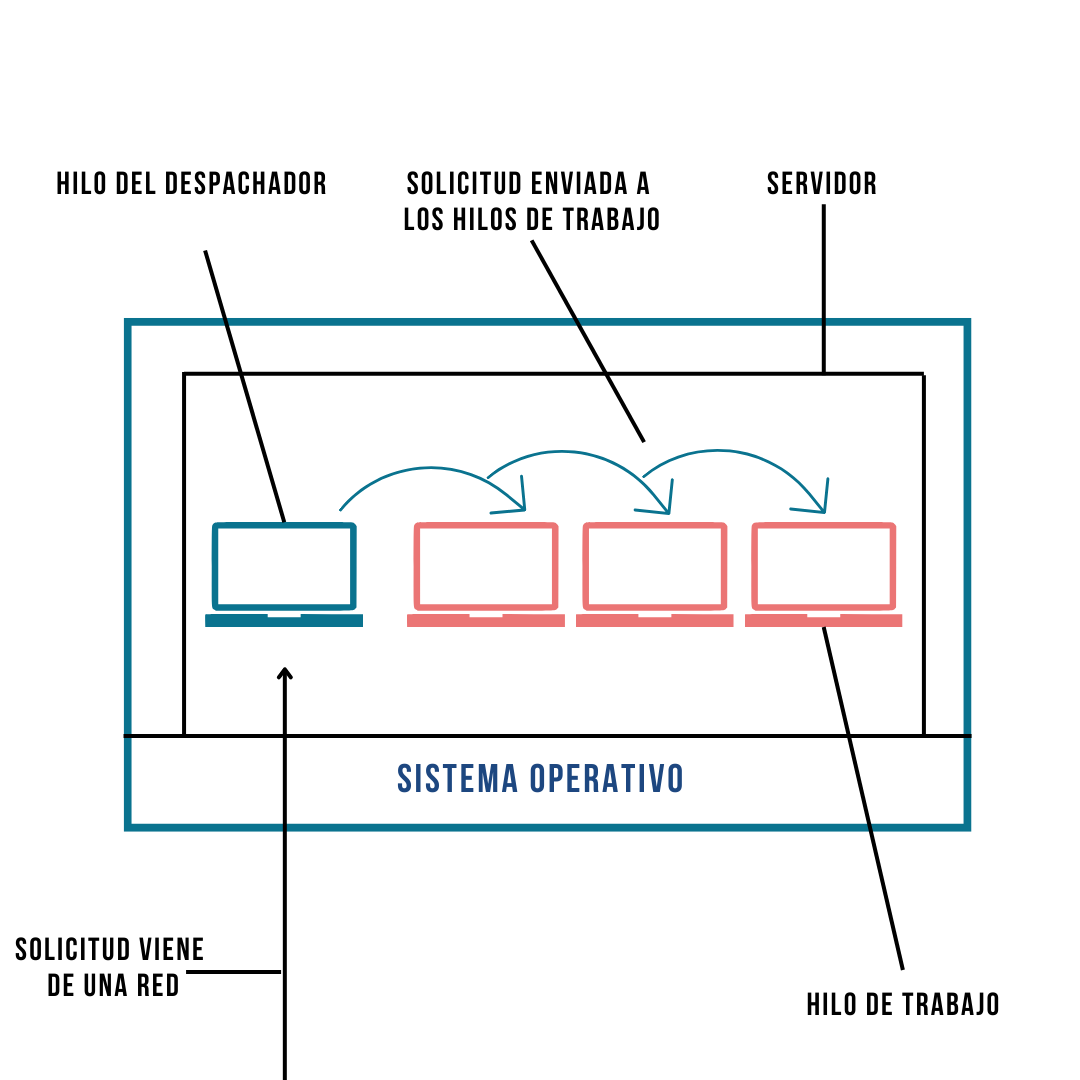
\includegraphics[width=0.9\linewidth]{3/14.png}
		\caption{Servidor Multihilo. }
		\label{fig:serv-multi}
	\end{figure}

 
 %%%%%%
 \paragraph*{Arquitectura para servidores multihilos}
 En la arquitectura de hilos por solicitud (Figura \ref{fig:hilo-sol-1}), el hilo de E/S genera un nuevo hilo de trabajo por cada solicitud, y ese hilo trabajador se destruye a sí mismo cuando ha procesado la  solicitud contra el objeto remoto designado. Esta arquitectura tiene la ventaja de que  los hilos no compiten por una cola compartida y el rendimiento se maximiza potencialmente  ya que el hilo de E/S puede crear tantos hilos trabajadores como solicitudes pendientes.  La desventaja es la sobrecarga de las operaciones en la creación y destrucción de hilos.
 		 
 		 \begin{figure} %
 			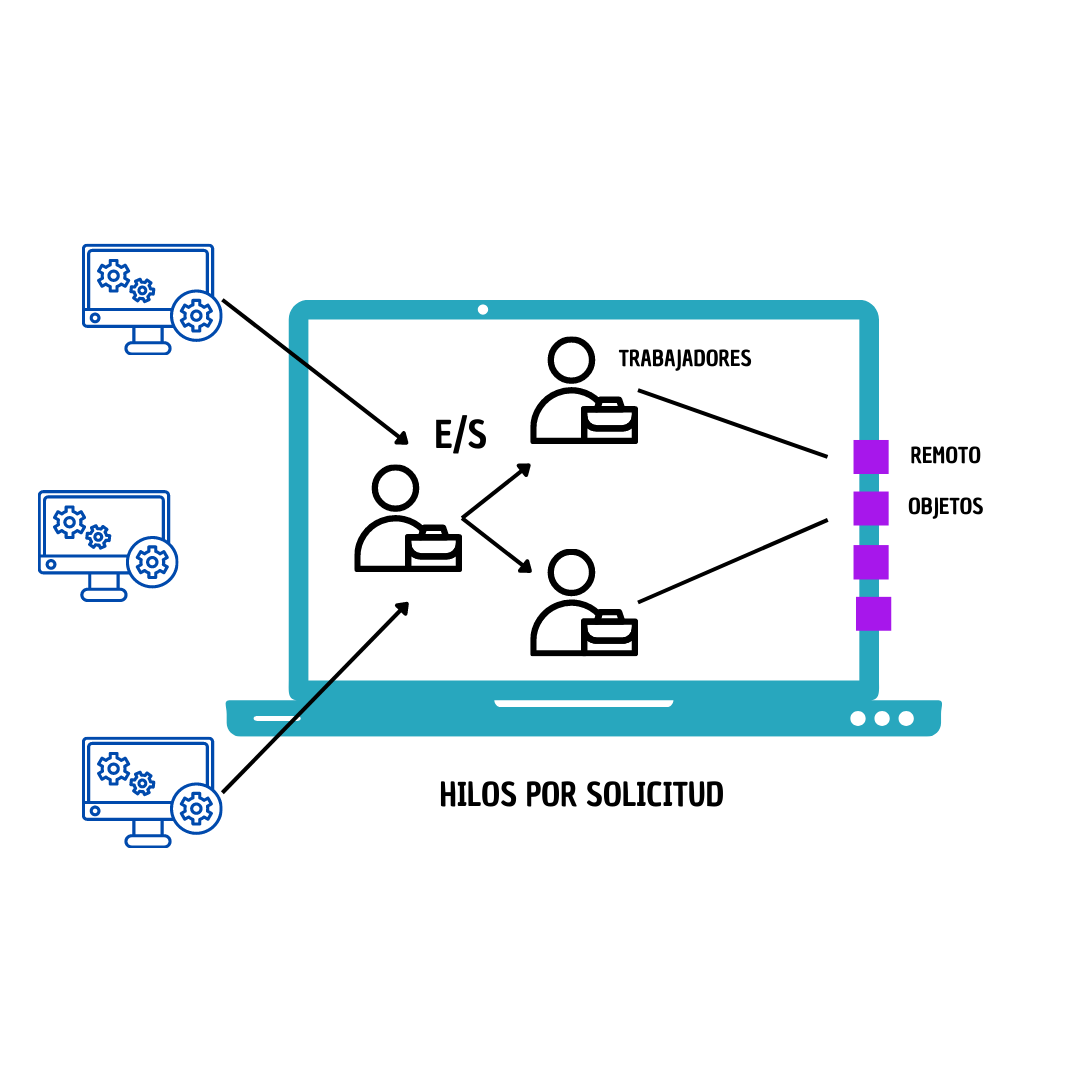
\includegraphics{3/2}  		 	 	 
 	\caption{Servidores multihilos por solicitud}
 	\label{fig:hilo-sol-1}
 \end{figure}
 
 
 La arquitectura hilo por conexión representado en la Figura \ref{fig:hilo-sol-2}, asocia un hilo con cada conexión. El servidor crea un nuevo hilo de trabajo cuando un cliente realiza una  conexión y destruye el hilo cuando el cliente cierra la conexión. Mientras tanto, el cliente puede realizar muchas solicitudes a través de la conexión, dirigidas a uno o más objetos remotos. 

 \begin{figure}%
 	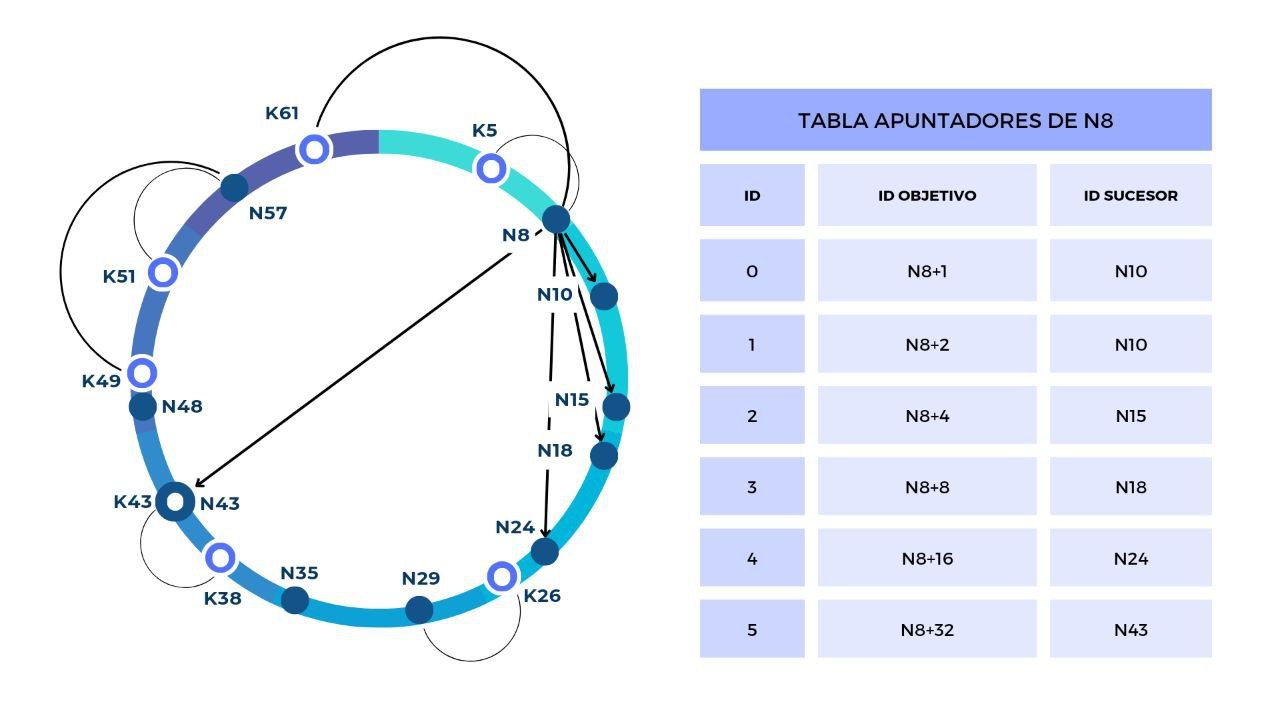
\includegraphics{3/3} 	 
	\caption{Servidores multihilos por conexi\'on}
	\label{fig:hilo-sol-2}
\end{figure}
 
  La arquitectura hilo por objeto en la Figura \ref{fig:hilo-sol-3}, asocia un hilo con cada  objeto remoto. Un subproceso de E/S recibe solicitudes y las pone en cola para los trabajadores, pero esta vez hay una cola por objeto.
   
    \begin{figure} %
   	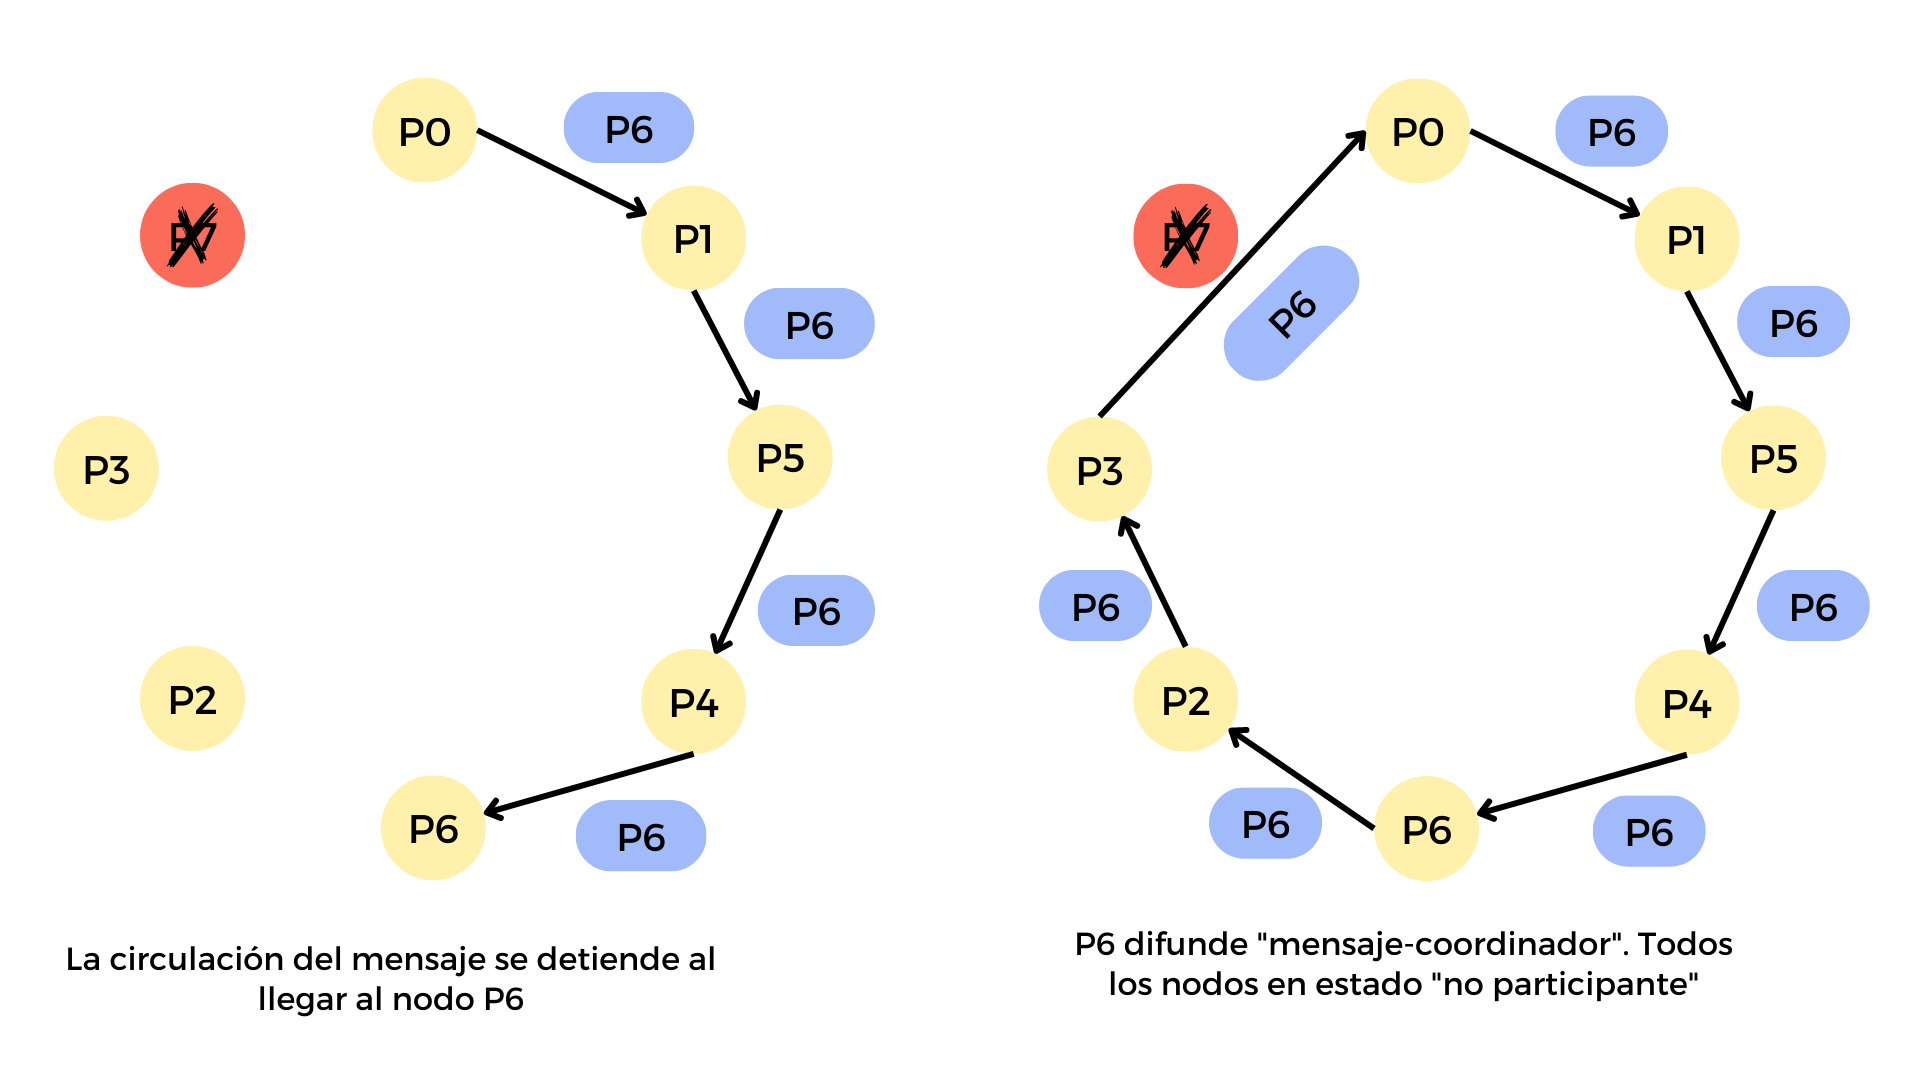
\includegraphics{3/4} 	 
   	\caption{Servidores multihilos por objeto}
   	\label{fig:hilo-sol-3}
   \end{figure}
 
En cada una de estas dos últimas arquitecturas, el servidor se beneficia de una gestión de hilos con bajo costo si se compara con la arquitectura de hilos por solicitud. Su desventaja es que los clientes pueden retrasarse mientras un hilo de trabajo tiene varios solicitudes pendientes pero otro hilo no tiene trabajo que realizar.

\marginnote[-4cm]{
	\begin{kaobox}[frametitle={Ejemplo de servidor multihilo}  ]
		En esta dirección \href{https://www.tutorialspoint.com/javaexamples/net_multisoc.htm}{Servidor multihilo} puede ver y ejecutar un servidor multihilo
	\end{kaobox}
}


%%%%%%%%%%%%%%%%%%%%

	
	%------------------------------------------------
	\section{Virtualizaci\'on de sistemas}   \index{virtualización}
	%------------------------------------------------
	La virtualización es una tecnología que se puede usar para crear representaciones virtuales de servidores, almacenamiento, redes y otras máquinas físicas.
	La virtualización puede ser aplicada en el contexto de la creación de \gls{redes superpuestas}, que ofrecen soporte para tipos particulares de aplicaciones  distribuidas. Otra aplicación es la virtualización de sistemas, que es en el contexto  de los sistemas operativos; esta es la que se estudia en esta sección. 
	
	El objetivo de la virtualización de sistema \sidecite{Coulouris2011} es proporcionar múltiples máquinas virtuales (imágenes de hardware virtual) sobre la arquitectura de la máquina física subyacente, con cada virtual máquina que ejecuta una instancia de sistema operativo separada. El concepto surge de la 	observación de que las arquitecturas informáticas modernas tienen el rendimiento necesario para 	admitir potencialmente un gran número de máquinas virtuales y recursos multiplexados entre
	a ellos. Varias instancias del mismo sistema operativo pueden ejecutarse en máquinas virtuales o se puede admitir una gama de diferentes sistemas operativos. El sistema de virtualización asigna los procesadores físicos y otros recursos de una máquina física entre todas las máquinas virtuales que admite.
	
	\paragraph{Tipos de Virtualización} 
	%%%%%%%%%%%%%%%%%%%%%%%%%
 
	
	En La Figura \ref{fig:virtualizacion-API} se  muestra, de acuerdo a \sidecite{Smith2005},  cuatro tipos de interfaces en tres niveles diferentes de las capas de implementación en un sistema informático típico: la arquitectura del conjunto de instrucciones (ISA, \textit{instruction set architecture}), la interfaz binaria de la aplicación (ABI, \textit{application binary interface}) y  interfaz de programación de aplicaciones (API, \textit{application programming interface}).
	
			 \begin{figure} %
		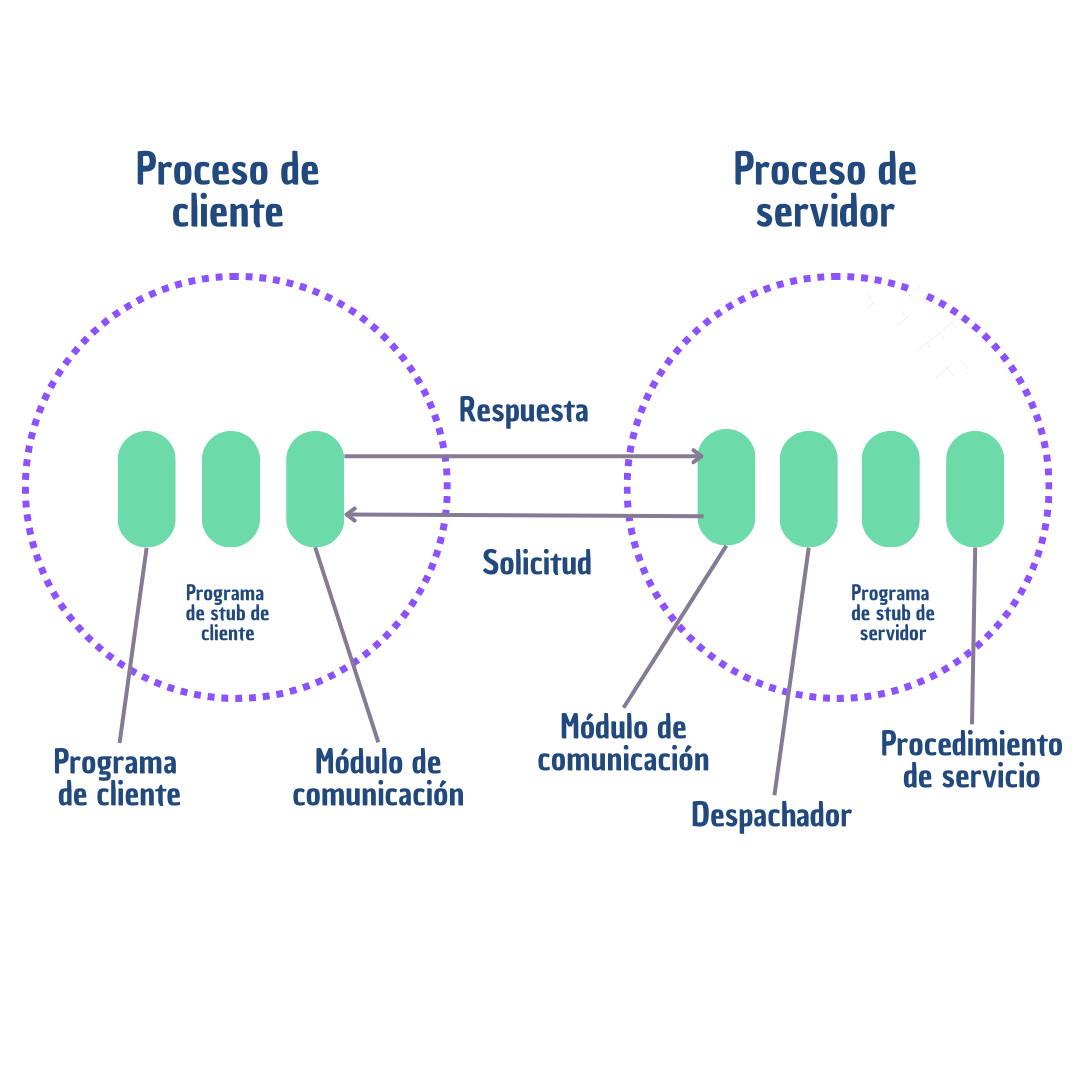
\includegraphics[width=10cm]{3/5}	 
		\caption{Interfases en sistemas informaticos. Adaptado  de \cite{Smith2005}}
		\label{fig:virtualizacion-API}
	\end{figure}
	
	
	\begin{itemize}
		\item ISA.  La ISA marca la división entre hardware y software, y consta de las interfaces: (a) la ISA del usuario e incluye aquellos aspectos visibles para un programa de aplicación (interfaz 4); (b)  es un superconjunto del usuario ISA e incluye aquellos aspectos visibles solo para el software del sistema operativo responsable de administrar los recursos de hardware, (interfaz 3).
	
		\item ABI. La ABI da acceso a un programa a los recursos y servicios de hardware disponibles en un sistema a través de la ISA de usuario (interfaz 4); y de la interfaz de llamada al sistema (interfaz 2).
	 
		\item API. La API le da a un programa acceso a los recursos y servicios de hardware disponibles en un sistema a través del usuario ISA (interfaz 4) complementado con llamadas de biblioteca de lenguaje de alto nivel (HLL) (interfaz 1). Cualquier llamada del sistema generalmente se realizan a través de bibliotecas.
	\end{itemize}

 
	%%%%%%%%%%%%%%%%%%%%%%%%%
	
	La esencia de la virtualización estriba en la capacidad de imitación de las interfaces mencionadas. En la figura \ref{fig:virtualizacion-tipo}   se ilustra las formas de virtualización.   
	
 
	\begin{enumerate}
		
		\item [(a)] Conjunto separado de instrucciones, un intérprete/emulador, que se ejecuta sobre un sistema operativo.
		Se puede construir un sistema en tiempo de ejecución que esencialmente proporcione un conjunto de instrucciones abstractas que se utilizará para ejecutar aplicaciones. Las instrucciones se pueden interpretarse (ejemplo, Java) o emularse  (emular SO Windows sobre Linux).
		
		\item [(b)] Instrucciones de bajo nivel, junto con un sistema operativo mínimo básico. 
		Este enfoque  se conoce como un monitor de máquina virtual nativo. Se llama nativo porque se implementa directamente en parte superior del hardware subyacente. Tenga en cuenta que la interfaz que ofrece un monitor de máquina virtual se puede ofrecer simultáneamente a diferentes programas. Tendría que proporcionar y regular el acceso
		a varios recursos, como almacenamiento externo y redes; esto implica que tendrá que implementar controladores de dispositivo para esos recursos. 		
		 Como resultado, ahora es posible tener múltiples y diferentes sistemas operativos invitados ejecutándose de forma independiente y simultánea en la misma plataforma.
		 
		
		
		\item [(c)] Instrucciones de bajo nivel, pero delegando la mayor parte del trabajo a un sistema operativo completo.	
		 Esta configuración llamada  monitor de máquina virtual alojada se ejecutará sobre un sistema operativo alojador (\textit{host}) de confianza, como se muestra en la Figura 3.8(c). En este caso, el monitor de la máquina virtual puede hacer uso de las instalaciones existentes proporcionadas por ese sistema operativo \textit{host}.
		
		
		
	\end{enumerate}
	
  %\begin{figure} %
% 	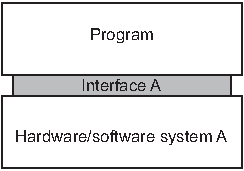
\includegraphics[width=4cm]{3/03-06a.pdf}  \hspace{2ex}
 %  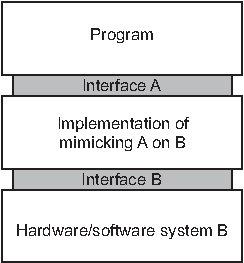
\includegraphics[width=4cm]{3/03-06b.pdf}
% 	\caption{Tipos de Virtualización . Adaptado  de \ST }
% 	\label{fig:virtualizacion-tipo}
% \end{figure}
 	%------------------------------------------------
 
		
		 \begin{figure} %
			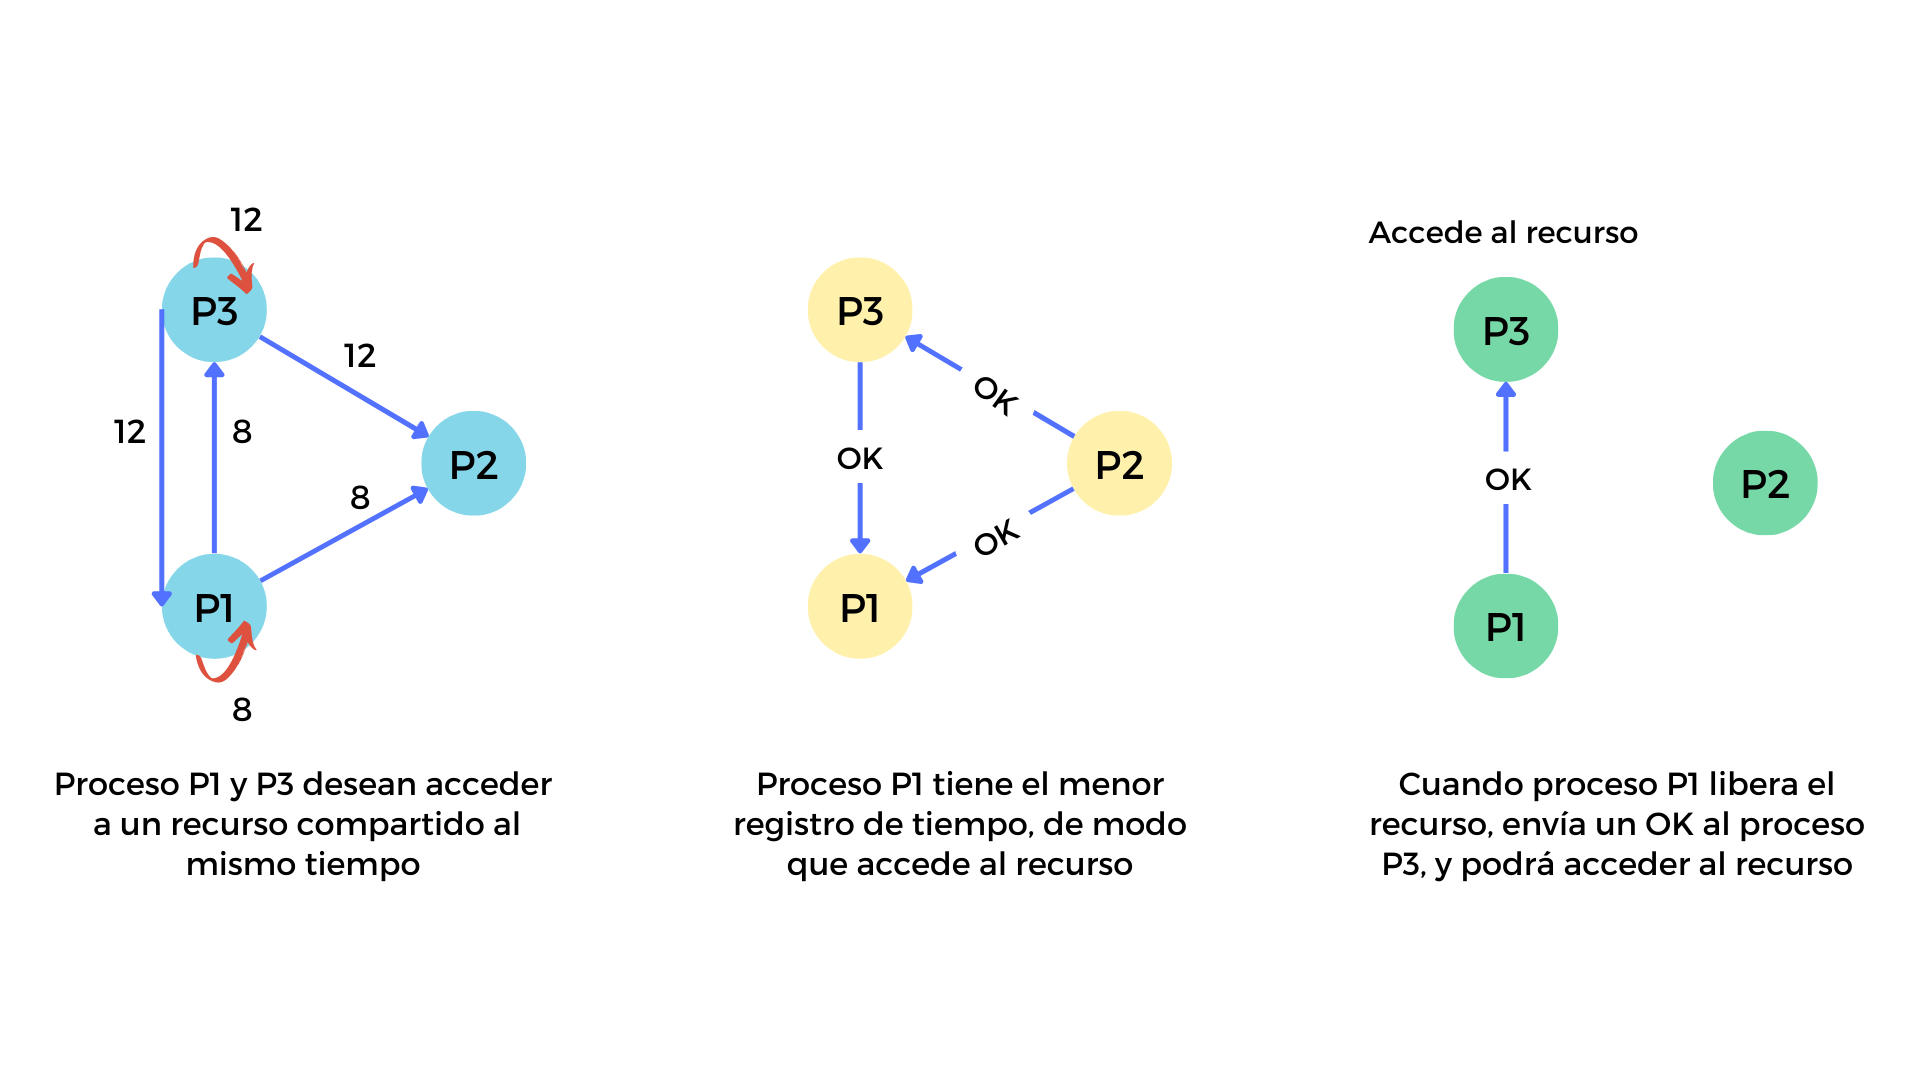
\includegraphics[width=3.5cm]{3/10}
			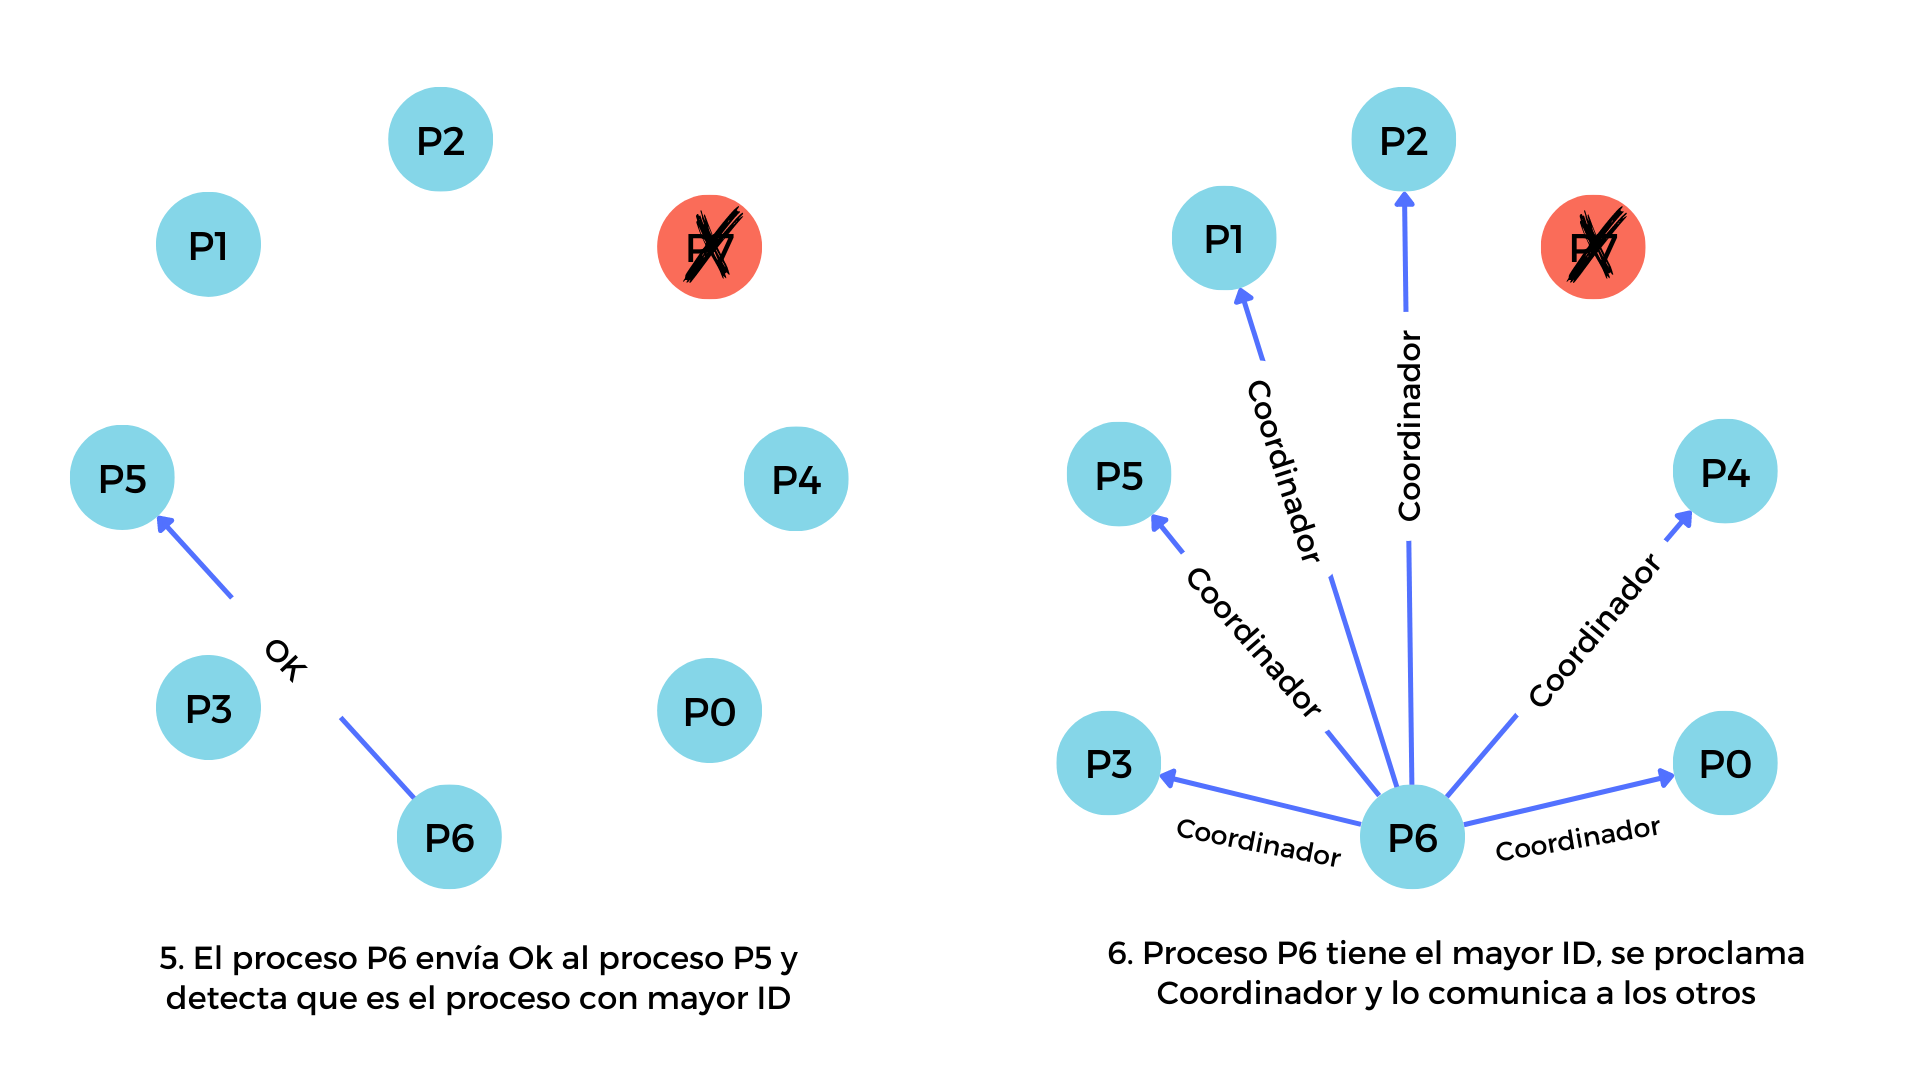
\includegraphics[width=3.5cm]{3/9}
			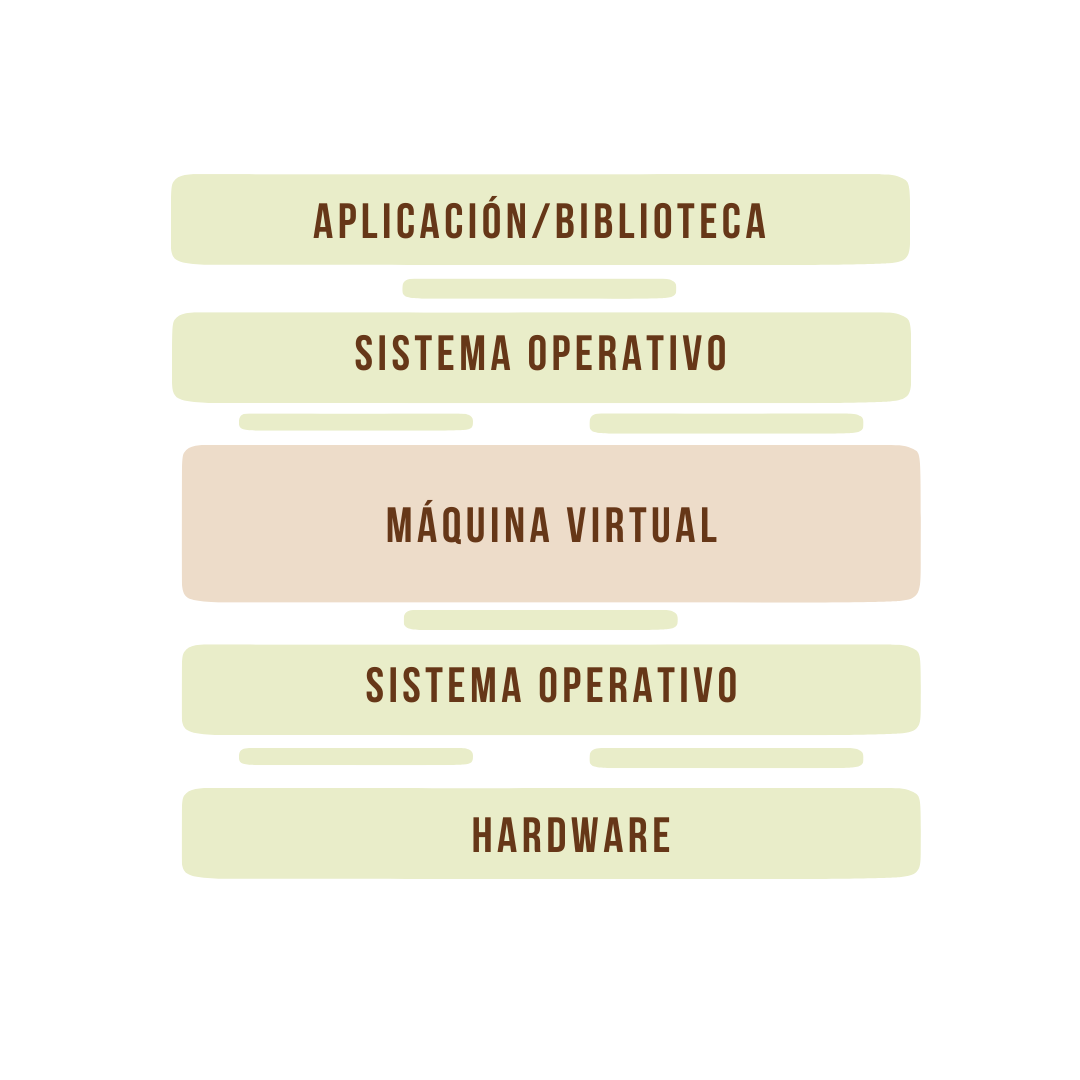
\includegraphics[width=3.5cm]{3/8}
			\caption{Formas de Virtualización: (a) VM de proceso, (b) VMM nativo, (c) VMM alojado. Adaptado  de \ST }
			\label{fig:virtualizacion-tipo}
		\end{figure}
		

	
	%-------------------------------------------------
\subsection{ VM y computación en la nube }
\index{virtualización}
		{Tres tipos de servicios en la nube \sidecite{Ozsu2020}		 
			\begin{itemize} 	
				\item \textbf{Infraestructura como servicio} que cubre la infraestructura básica				
				\item \textbf{Plataforma como servicio} que cubre servicios a nivel de sistema 			
				\item  \textbf{Software como servicio} que contiene aplicaciones reales
			\end{itemize}
		

 %%%%%%%%%
 
 \paragraph{Infraestructura como servicio (IaaS.)} IaaS es la distribución de una infraestructura informática  (recursos informáticos, de redes y de almacenamiento) como un servicio. Permite a los clientes escalar (agregar más recursos) o reducir (liberar recursos) cuando sea  necesarios (y solo pagan por los recursos consumidos). Esta  capacidad es  llamado \textbf{elasticidad} y generalmente se logra a través de la virtualización de servidores, una tecnología  que permite que varias aplicaciones se ejecuten en el mismo servidor físico que las máquinas virtuales, es decir, como si se ejecutaran en distintos servidores físicos. Luego, los clientes pueden solicitar instancias informáticas como máquinas virtuales y agregar y adjuntar almacenamiento según sea necesario. Un ejemplo de IaaS  son los servicios web de \textbf{\href{https://aws.amazon.com/es/}{Amazon}}. 
 \index{IaaS}
 \index{infraestructura como servicio}
 
\paragraph{Software como servicio (SaaS.)} SaaS es la entrega de software de aplicación como  un servicio. Generaliza el modelo anterior de proveedor de servicios de aplicaciones (ASP)  mediante el cual la aplicación alojada es propiedad exclusiva, operada y mantenida por el  ASP. Con SaaS, el proveedor de la nube permite al cliente utilizar aplicaciones alojadas
 (como con ASP) pero también proporciona herramientas para integrar otras aplicaciones, de diferentes  proveedores o incluso desarrollado por el cliente (usando la plataforma en la nube).
 Ejemplo de una SaaS   es el sistema \textbf{\href{https://www.salesforce.com/mx/?ir=1}{Safesforce CRM}}.
 \index {SaaS}
  \index{software como servicio}
 
 \paragraph{Plataforma como servicio (PaaS.)} PaaS es la entrega de una plataforma informática  con herramientas de desarrollo y APIs como servicio. Permite a los desarrolladores crear  e implementar aplicaciones personalizadas directamente en la infraestructura de la nube e integrarlas con aplicaciones proporcionadas como SaaS. Un ejemplo de  PaaS   es \textbf{\href{https://play.google.com/store/apps?hl=es_VE&gl=US}{Google Apps}}.
 \index{PaaS}
  \index{plataforma como servicio}
 
 \section{Caso de Estudio: Virtualización de Redes}
 \index{caso de estudio!virtualización de redes}
 \label{sec:redes-sup}
 
La Virtualización de redes  e ocupa de la construcción de  redes virtuales diferentes a través de una red base existente como la red de Internet. Cada  red virtual se puede diseñar para admitir una aplicación distribuida en particular \sidecite{Coulouris2011}.
 
 Por ejemplo, una red virtual podría admitir la transmisión de multimedia, como en \href{https://www.youtube.com/}{Youtube}, 
 \href{https://www.netflix.com/ve/}{Netflix}    y convivir con otras redes que admita un juego con múltiples jugadores  en línea; todos estos ejemplos se ejecutan en la misma red subyacente. Una red virtual específica para una aplicación se puede construir sobre la red existente y
 se optimiza para esa aplicación en particular, sin cambiar las características del red subyacente. 
 
 Las  \gls{redes superpuestas} son redes virtuales (\sidecite{Peterson2021}) que consta de nodos y enlaces virtuales, que se encuentra encima de una red subyacente (como una red IP), en la figura \ref{fig:red-overlay} se muestra un esquema de una red superpuesta.
 
 	\begin{figure}%
 	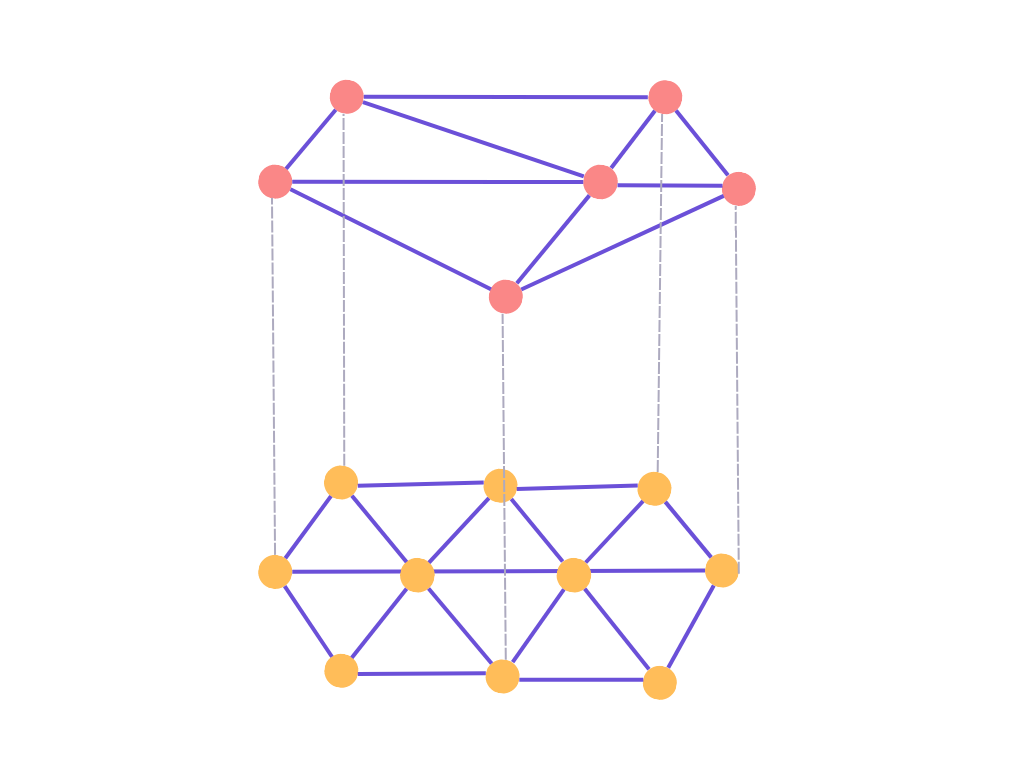
\includegraphics{3/17.png}
 	\caption{Red Superpuesta.}
 	\label{fig:red-overlay}
 \end{figure}
 
 
  Las redes superpuestas ofrecen:   
 \begin{itemize}
 	\item   un servicio que se adapta a las necesidades de una clase de aplicación o un servicio particular  nivel superior, por ejemplo, las redes sociales;
 	\item  una operación más eficiente en un entorno de red determinado, por ejemplo, enrutamiento en una red específica;
 	\item  una función adicional, por ejemplo, multidifusión o comunicación segura.
 \end{itemize}   \index{red superpuesta} 
 
% Las redes superpuestas tienen las siguientes ventajas:  \index{red superpuesta!ventaja}
% \begin{itemize} 
 %	\item  Permiten definir nuevos servicios de red sin requerir cambios en la red subyacente, un punto crucial dado el nivel de estandarización en esta área y las dificultades de modificar la funcionalidad de enrutadores subyacente.  	\item Fomentan la experimentación con servicios de red y la personalización de servicios a clases particulares de aplicación.  	\item Se pueden definir múltiples superposiciones las cuales  pueden coexistir,  proporcionando una  Arquitectura de red abierta y extensible.  \end{itemize}
 
 %%Las desventajas son que las superposiciones introducen un nivel adicional de no-dirección (y por lo tanto puede incurrir en una penalización de rendimiento) y se suman a la complejidad de los servicios de red  en comparación, por ejemplo, con la arquitectura relativamente simple de las redes TCP / IP.\index{red superpuesta!desventaja}
 
 Ejemplo de redes superpuesta se encuentra: Skype,   redes sociales, redes inalámbricas  y redes tolerantes a las interrupciones en el contexto de los dispositivos móviles y
 computación ubicua,  y  el  soporte de superposición para transmisión multimedia.
 
 \subsection{Skype: un ejemplo de una red superpuesta}
 \index{Skype} \label{Skype}
 \href{https://www.skype.com}{Skype} es una aplicación P2P que ofrece voz sobre IP (\textit{VoIP}) \sidecite{Baset2006}. También incluye mensajería instantánea, videoconferencia e interfaces para el servicio de telefonía estándar a través de \textit{SkypeIn} y \textit{SkypeOut}.  
 \marginnote[3cm]{
 	\begin{kaobox}[frametitle= Skype ]
 		El software fue desarrollado por Kazaa en 2003 y por lo tanto, comparte muchas de las características del intercambio de archivos entre pares de la aplicaci\'on  Kazaa \cite{Leibowitz2003} 
 	\end{kaobox}
 }
  
 Skype es una red virtual en el sentido de que establece conexiones entre personas (suscriptores de Skype activos). No se requiere ninguna dirección IP o puerto para establecer una llamada.

 
 \begin{description}  \index{arquitetura de Skype}
 	\item[Arquitectura de Skype]  Skype se basa en una infraestructura P2P que consta de  máquinas de usuarios comunes (\textit{hosts}) y supernodos: los supernodos son \textit{hosts} de Skype ordinarios que tienen capacidades suficientes para llevar a cabo su funci\'on. Los supernodos se seleccionan a pedido, en función  de criterios que incluyen ancho de banda disponible, accesibilidad (la máquina debe tener una dirección IP global y no  oculto detrás de un enrutador habilitado para NAT, por ejemplo) y disponibilidad (según el tiempo que Skype se ha estado ejecutando en ese nodo). Esta estructura general   	se captura en la Figura \ref{fig:skype} .
 	
 	
 	\begin{figure}%
 		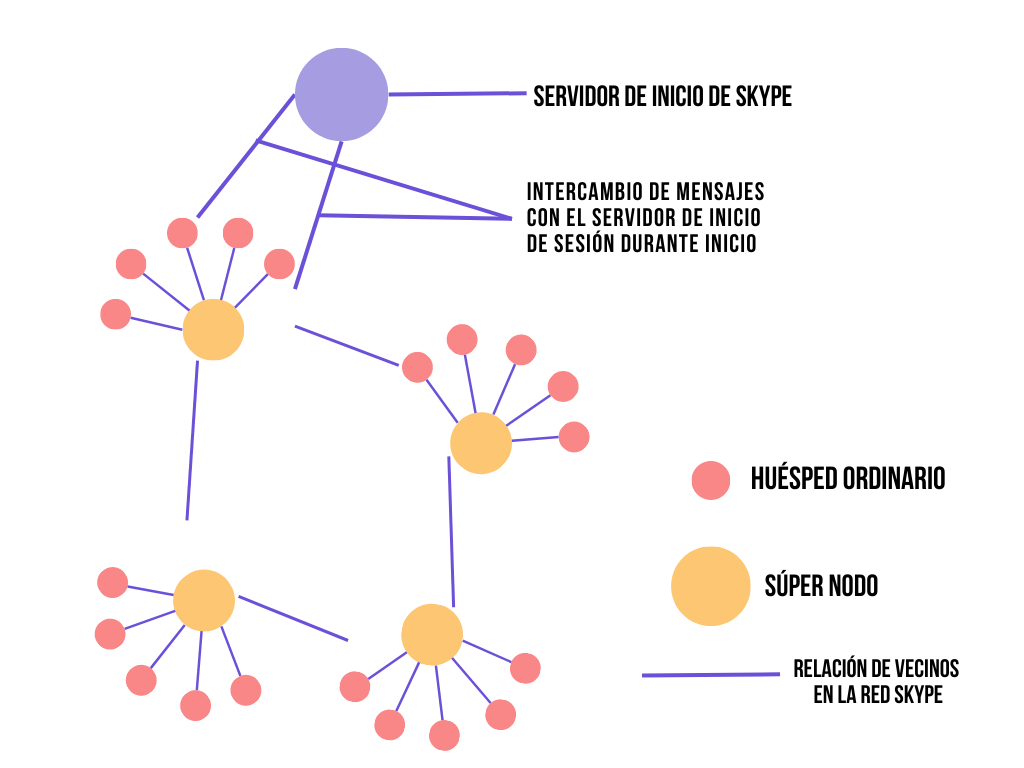
\includegraphics{3/16.png}
 		\caption{Arquitectura Skype.}
 		\label{fig:skype}
 	\end{figure}
 	
 	\item[Conexión de usuario]  Los usuarios de Skype se autentican a través de un conocido servidor de inicio de sesión. Luego contacta con un supernodo seleccionado. Para lograrlo, cada cliente mantiene un caché de identidades de supernodo (es decir, pares de direcciones IP y números de puerto). En el primer inicio de sesión este caché se llena con las direcciones de alrededor de siete supernodos, y con el tiempo el  cliente crea y mantiene un conjunto mucho más grande (quizás varios cientos).
 	
 	\item[Búsqueda de usuarios]  El objetivo principal de los supernodos es realizar la búsqueda eficiente de los índices globales de usuarios, que se distribuye entre los supernodos. La busqueda es orquestada por el supernodo elegido por el cliente e implica una búsqueda en expansión de otros super nodos hasta que se encuentre el usuario especificado. En promedio, se contactan ocho supernodos. La búsqueda de un usuario suele tardar entre tres y cuatro segundos en completarse en los \textit{hosts} que tienen una dirección IP global (y un poco más larga, de cinco a seis segundos, si están detrás de un enrutador habilitado para NAT). De acuerdo a los experimentos de  \sidecite{Baset2006}, parece que los nodos intermediarios involucrados en la búsqueda, almacenan en caché los resultados para mejorar el rendimiento.
 	
 	\item[Conexión de voz]  Una vez que se encuentra  al usuario requerido, Skype establece una conexión de voz entre las dos partes utilizando TCP para señalizar solicitudes de llamada,  y UDP o TCP para la transmisión de audio. Se prefiere UDP en vez de TCP. El software utilizado para codificar y decodificar audio juega un papel clave para proporcionar una excelente calidad de llamada que normalmente se logra con Skype, y los algoritmos asociados se adaptan cuidadosamente a operar en entornos de Internet a 32 kbps y superiores.
 	
 \end{description}
 
 